\documentclass[10pt,a4paper,twoside]{article}
\usepackage{pstricks}
\usepackage{fancybox}
\usepackage{amsfonts}
% \usepackage{minitoc}
% \setcounter{minitocdepth}{2}
\usepackage[bookmarks=true, 
            bookmarksnumbered=true, 
            bookmarksopen=false, 
            plainpages=false,
            pdfpagelabels,
            colorlinks, 
            linkcolor=blue]{hyperref}
\usepackage{ifthen}
\usepackage{graphicx}
\newtheorem{theorem}{Theorem}
\newtheorem{corollary}{Corollary}

%\newboolean{mtc}
%\setboolean{mtc}{true}

\pdfoutput=1
\relax
\pdfcompresslevel=0             %-- 0 = none, 9 = best
\pdfinfo{                       %-- Info dictionary of PDF output  /Author (Alfredo Buttari)
  /Title (  MultiLevel Domain Decomposition Parallel Preconditioners Package
             based on PSBLAS V. 1.0)
  /Subject ( MultiLevel Domain Decomposition Parallel Preconditioners
  Package)
  /Keywords (Computer Science Linear Algebra Fluid Dynamics Parallel Linux MPI PSBLAS Iterative Solvers Preconditioners)
  /Creator (pdfLaTeX)
  /Producer ($Id: userguide.tex 1978 2007-10-19 14:51:12Z sfilippo $)
}
\pdfcatalog{          %-- Catalog dictionary of PDF output.
  /URI (http://ce.uniroma2.it/psblas)
} 

\newcounter{subroutine}[subsection]
\newcounter{example}[subroutine]
\makeatletter
\def\subroutine{\@ifstar{\@subroutine}{\clearpage\@subroutine}}%
\def\@subroutine#1#2{%
\stepcounter{subroutine}%
      \section*{\flushleft #1---#2 \endflushleft}%
      \addcontentsline{toc}{subsection}{#1}%
      \markright{#1}}%
\newcommand{\subsubroutine}[2]{%
\stepcounter{subroutine}%
      \subsection*{\flushleft #1---#2 \endflushleft}%
      \addcontentsline{toc}{subsubsection}{#1}%
      \markright{#1}}%
\newcommand{\examplename}{Example}
\newcommand{\syntaxname}{Syntax}
\def\syntax{\@ifstar{\@ssyntax}{\@syntax}}%
\def\@syntax{\nobreak\section*{\syntaxname}%
     \@ssyntax}%
\def\@ssyntax#1#2{%
  \nobreak
   \setbox\@tempboxa\hbox{#1\ {\em $($#2$)$}}%
   \ifdim \wd\@tempboxa >\hsize
        \setbox\@tempboxa\hbox{\em $($#2$)$}
	\ifdim\wd\@tempboxa >\hsize
          \begin{flushright}#1\ \em$($#2$)$\end{flushright}%
	\else
         \hbox to\hsize{#1\hfil}%
         \hbox to\hsize{\hfil\box\@tempboxa}%
        \fi
     \else
       \hbox to\hsize{\hfil\box\@tempboxa\hfil}%
   \fi\par\vskip\baselineskip}
\makeatother
\newcommand{\example}{\stepcounter{example}%
\section*{\examplename~\theexample}}

\newcommand{\precdata}{\hyperlink{precdata}{{\tt mld\_prec\_type}}}
\newcommand{\descdata}{\hyperlink{descdata}{{\tt psb\_desc\_type}}}
\newcommand{\spdata}{\hyperlink{spdata}{{\tt psb\_spmat\_type}}}

\begin{document}
%%%%%%%%%%%%%%%%%%%%%%%%%%%%%%%%%%%%%%%%%%%%%%%%%%%%%%%%%%%%%%%%%
% Contents: The title page
% $Id: title.tex 1999 2007-10-29 15:25:27Z sfilippo $
%%%%%%%%%%%%%%%%%%%%%%%%%%%%%%%%%%%%%%%%%%%%%%%%%%%%%%%%%%%%%%%%%

\ifx\pdfoutput\undefined % We're not running pdftex
\else
\pdfbookmark{MLD2P4-1.0 User's Guide}{title}
\fi
\newlength{\centeroffset}
\setlength{\centeroffset}{-0.5\oddsidemargin}
\addtolength{\centeroffset}{0.5\evensidemargin}
%\addtolength{\textwidth}{-\centeroffset}
\thispagestyle{empty}
\vspace*{\stretch{1}}
\noindent\hspace*{\centeroffset}\makebox[0pt][l]{\begin{minipage}{\textwidth}
\flushright
{\Huge\bfseries MLD2P4-1.0 User's guide
}
\noindent\rule[-1ex]{\textwidth}{5pt}\\[2.5ex]
\hfill\emph{\Large A reference guide for the MultiLevel Domain
  Decomposition Parallel Preconditioners Package based on Parallel Sparse BLAS}
\end{minipage}}

\vspace{\stretch{1}}
\noindent\hspace*{\centeroffset}\makebox[0pt][l]{\begin{minipage}{\textwidth}
\flushright
{\bfseries 
by Salvatore Filippone\\
   Alfredo Buttari} \\
University of Rome ``Tor Vergata'' \\[3ex]
{\bfseries Daniela di Serafino }\\
Second University of Naples\\[3ex]
{\bfseries Pasqua D'Ambra}\\
ICAR-CNR, Naples\\[3ex]
\today
\end{minipage}}

%\addtolength{\textwidth}{\centeroffset}
\vspace{\stretch{2}}

\endinput

%

% Local Variables:
% TeX-master: "userguide"
% mode: latex
% mode: flyspell
% End:


\cleardoublepage
\begingroup
  \renewcommand*{\thepage}{toc}
  \pagenumbering{roman}   % Roman numbering
  \setcounter{page}{1}    % Abstract start on page ii
  \tableofcontents
\endgroup  

\cleardoublepage

\pagenumbering{arabic}  % Arabic numbering
\setcounter{page}{1}    % Chapters start on page 1

\section{Introduction}

The PSBLAS library, developed with the aim to facilitate the
parallelization of computationally intensive scientific applications,
is designed to address parallel implementation of iterative solvers
for sparse linear systems through the distributed memory paradigm.  It
includes routines for multiplying sparse matrices by dense matrices,
solving block diagonal systems with triangular diagonal entries,
preprocessing sparse matrices, and contains additional routines for
dense matrix operations.  The current implementation of PSBLAS
addresses a distributed memory execution model operating with message
passing. 

The PSBLAS library is internally implemented in a mixture of
Fortran~77 and Fortran~95~\cite{metcalf} programming languages. A
similar approach has been advocated by a number of authors,
e.g.~\cite{machiels}.  Moreover, the Fortran~95 facilities for dynamic
memory management and interface overloading greatly enhance the usability of the PSBLAS
subroutines. In this way, the library can take care of runtime memory
requirements that are quite difficult or even impossible to predict at
implementation or compilation time.  The following presentation of the
PSBLAS library follows the general structure of the proposal for
serial Sparse BLAS~\cite{sblas97,sblas02}, which in its turn is based on the
proposal for BLAS on dense matrices~\cite{BLAS1,BLAS2,BLAS3}.

The applicability of sparse iterative solvers to many different areas
causes some terminology problems because the same concept may be
denoted through different names depending on the application area. The
PSBLAS features presented in this section will be discussed mainly in terms of finite
difference discretizations of Partial Differential Equations (PDEs).
However, the scope of the library is wider than that: for example, it
can be applied to finite element discretizations of PDEs, and even to
different classes of problems such as nonlinear optimization, for
example in optimal control problems.

The design of a solver for sparse linear systems is driven by many
conflicting objectives, such as limiting occupation of storage
resources, exploiting regularities in the input data, exploiting
hardware characteristics of the parallel platform.  To achieve an
optimal communication to computation ratio on distributed memory
machines it is essential to keep the {\em data locality} as high as
possible; this can be done through an appropriate data allocation
strategy.  The choice of the preconditioner is another very important
factor that affects efficiency of the implemented application. Optimal
data distribution requirements for a given preconditioner may conflict
with distribution requirements of the rest of the solver. Finding the
optimal trade-off may be very difficult because it is application
dependent.  Possible solution to these problems and other important
inputs to the development of the PSBLAS software package has come from
an established experience in applying the PSBLAS solvers to
computational fluid dynamics applications.

\section{General overview}
\label{sec:overview} 
The PSBLAS library is designed to handle the implementation of
iterative solvers for sparse linear systems on distributed memory
parallel computers.  The system coefficient matrix $A$ must be square;
it may be real or complex, nonsymmetric, and its sparsity pattern
needs not to be symmetric.  The serial computation parts are based on
the serial sparse BLAS, so that any extension made to the data
structures of the serial kernels is available to the parallel
version. The overall design and parallelization strategy have been
influenced by the structure of the ScaLAPACK parallel
library.  The layered structure of the PSBLAS library
is shown in figure~\ref{fig:psblas} ; lower layers of the library
indicate an encapsulation relationship with upper layers. The ongoing
discussion focuses on the Fortran~95 layer immediately below the
application layer.
The serial parts of the computation on each process are executed through
calls to the serial sparse BLAS subroutines. In a similar way, the
inter-process message exchanges are implemented through the Basic
Linear Algebra Communication Subroutines (BLACS) library~\cite{BLACS}
that guarantees a portable and efficient communication layer. The
Message Passing Interface code is encapsulated within the BLACS
layer. However, in some cases, MPI routines are directly used either
to improve efficiency or to implement communication patterns for which
the BLACS package doesn't provide any method. 
We assume that the user program has initialized a BLACS process grid
with one column and as many rows as there are processes; the PSBLAS
initialization routines will take the communication context for this
grid and store internally for further use. 

\begin{figure}[h] \begin{center}
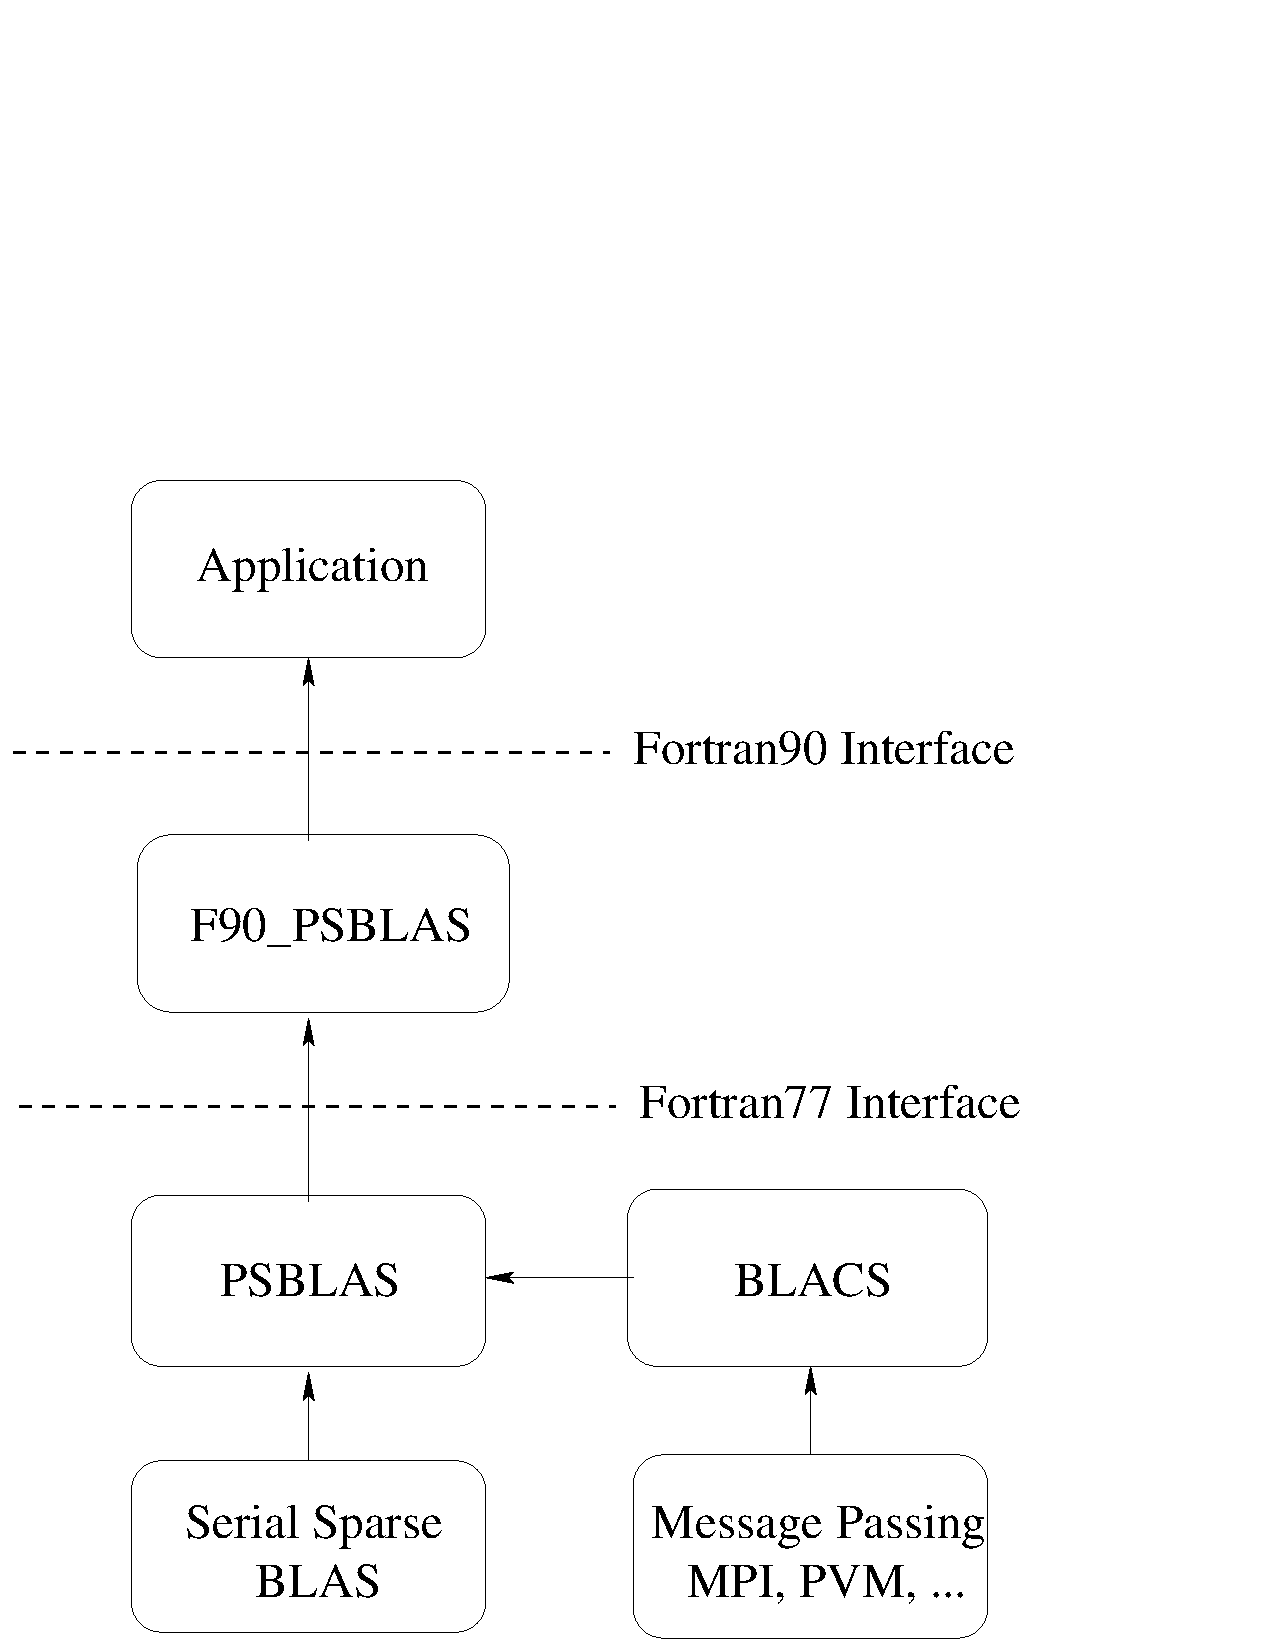
\includegraphics[scale=0.45]{figures/psblas}
\end{center}
\caption{PSBLAS library components hierarchy.\label{fig:psblas}}
\end{figure}

The PSBLAS library consists of two classes of subroutines that is, the
{\em computational routines} and the {\em auxiliary routines}.  The
computational routine set includes:
\begin{itemize}
\item Sparse matrix by dense matrix product; \item Sparse triangular
systems solution for block diagonal matrices;
\item Vector and matrix norms;
\item Dense matrix sums;
\item Dot products.
\end{itemize} 
The auxiliary routine set includes:
\begin{itemize}
\item Communication descriptors allocation;
\item Dense and sparse matrix allocation;
\item Dense and sparse matrix build and update;
\item Sparse matrix and data distribution preprocessing.
\end{itemize} 

The following naming scheme has been adopted for all the symbols
internally defined in the PSBLAS software package:
\begin{itemize}
\item all the symbols (i.e. subroutine names, data types...) are
  prefixed by \verb|psb_| 
\item all the data type names are suffixed by \verb|_type|
\item all the constant values are suffixed by \verb|_|
\item all the subroutine names follow the rule \verb|psb_xxname| where
  \verb|xx| can be either:
  \begin{itemize}
  \item \verb|ge|: the routine is related to dense data, 
  \item \verb|sp|: the routine is related to sparse data, 
  \item \verb|cd|: the routine is related to communication descriptor (see~\ref{sec:datastruct}).
  \end{itemize}
  For example the \verb|psb_geins|, \verb|psb_spins| and
  \verb|psb_cdins| perform the same action (see~\ref{sec:toolsrout}) on
  dense matrices, sparse matrices and communication descriptors
  respectively.
  Interface overloading allows the usage of the same subroutine
  interfaces for both real and complex data.
\end{itemize}
In the description of the subroutines, arguments or argument entries
are classified as:
\begin{description}
\item[global] For input arguments, the value must be the same on all processes
  participating in the subroutine call; for output arguments the value
  is guaranteed to be the same.
\item[local] Each process has its own value(s) independently.
\end{description}

\subsection{Application structure}

The main underlying principle of the PSBLAS library is that the
library objects are created and exist with reference to a discretized
space to which there corresponds an index space and a matrix sparsity
pattern. As an example, consider a cell-centered finite-volume
discretization of  the Navier-Stokes equations on a simulation domain;
the index space $1\dots n$ is isomorphic to the set of cell centers,
whereas the pattern of the associated linear system matrix is
isomorphic to the adjacency graph imposed on the discretization mesh
by the discretization stencil. 

Thus the first order of business is to establish an index space, and
this is done with a call to  \verb|psb_cdall| in which we specify the
size of the index space $n$ and the allocation of the elements of the
index space to the various processes making up the MPI (virtual)
parallel machine. 

The index space is partitioned among processes, and this creates a
mapping from the ``global'' numbering $1\dots n$ to a numbering
``local'' to each process; each process $i$ will own a certain subset
$1\dots n_{\hbox{row}_i}$, each element of which corresponds to a certain
element of $1\dots n$. The user does not set explicitly this mapping;
when the application needs to indicate to which element of the index
space a certain item is related, such as the row and column index of a
matrix coefficient, it does so in the ``global'' numbering, and the
library will translate into the appropriate ``local'' numbering. 

For  a given index space $1\dots n$ there are many possible associated
topologies, i.e. many different discretization stencils; thus the
description of the index space is not completed until the user has
defined a sparsity pattern, either explicitly through \verb|psb_cdins|
or implicitly through \verb|psb_spins|. The descriptor is finalized
with a call to \verb|psb_cdasb| and a sparse matrix with a call to
\verb|psb_spasb|. After \verb|psb_cdasb| each process $i$ will have
defined a set of ``halo'' (or ``ghost'') indices
$n_{\hbox{row}_i}+1\dots n_{\hbox{col}_i}$, denoting elements of the index
space that are \emph{not} assigned to process $i$; however the
variables associated with them are needed to complete computations
associated with the sparse matrix $A$, and thus they have to be
fetched from (neighbouring) processes. The descriptor of the index
space is built exactly for the purpose of properly sequencing the
communication steps required to achieve this objective. 

A simple application structure will walk through the index space
allocation, matrix/vector creation and linear system solution as
follows:
\begin{enumerate}
\item Initialize parallel environment with \verb|blacs_gridinit|
\item Initialize index space with \verb|psb_cdall|
\item Allocate sparse matrix and dense vectors with \verb|psb_spall|
  and \verb|psb_geall|
\item Loop over all local rows, generate matrix and vector entries,
  and insert them with \verb|psb_spins| and \verb|psb_geins|
\item Assemble the various entities: 
\begin{enumerate}
\item \verb|psb_cdasb|
\item \verb|psb_spasb|
\item \verb|psb_geasb|
\end{enumerate}
\item Choose the preconditioner to be used with \verb|psb_precset| and
  build it with \verb|psb_precbld|
\item Call the iterative method of choice, e.g. \verb|psb_bicgstab|
\end{enumerate}
This is the structure of the sample program
\verb|test/pargen/ppde90.f90|. 

For a simulation in which the same discretization mesh is used over
multiple time steps, the following structure may be more appropriate:
\begin{enumerate}
\item Initialize parallel environment with \verb|blacs_gridinit|
\item Initialize index space with \verb|psb_cdall|
\item Loop over the topology of the discretization mesh and build the
  descriptor with \verb|psb_cdins|
\item Assemble the descriptor with \verb|psb_cdasb|
\item Allocate the sparse matrices and dense vectors with
  \verb|psb_spall| and \verb|psb_geall|
\item Loop over the time steps: 
\begin{enumerate}
\item If after first time step, 
  reinitialize the sparse matrix with \verb|psb_sprn|; also zero out
  the dense vectors;
\item Loop over the mesh, generate the coefficients and insert/update
  them with \verb|psb_spins| and \verb|psb_geins|
\item Assemble with \verb|psb_spasb| and \verb|psb_geasb|
\item Choose and build preconditioner with \verb|psb_precset| and
  \verb|psb_precbld|
\item Call the iterative method of choice, e.g. \verb|psb_bicgstab|
 \end{enumerate}
\end{enumerate}
The insertion routines will be called as many times as needed; it is
clear that they only need be called on the data that is actually
allocated to the current process, i.e. each process generates its own
data. 

In principle there is no specific order in the calls to
\verb|psb_spins|, nor is there a requirement to build a matrix row in
its entirety before calling the routine; this allows the application
programmer to walk through the discretization mesh element by element,
generating the main part of a given matrix row but also contributions
to the rows corresponding to neighbouring elements. 

From a functional point of view it is even possible to execute one
call for each nonzero coefficient; however this would have a
substantial computational overhead. It is therefore advisable to pack
a certain amount of data into each call to the insertion routine, say
touching on a few tens of rows; the best performng value would depend
on both the architecture of the computer being used and on the problem
structure. 
At the opposite extreme, it would be possible to generate the entire
part of a coefficient matrix residing on a process and pass it in a
single call to \verb|psb_spins|; this, however, would entail a
doubling of memory occupation, and thus would be almost always far
from optimal. 

\subsection{Programming model}

The PSBLAS librarary is based on the Single Program Multiple Data
(SPMD) programming model: each process participating in the
computation performs the same actions on a chunk of data. Parallelism
is thus data-driven. 

Because of this structure, practically all subroutines \emph{must} be
called simultaneously by all processes participating in the
computation, i.e each subroutine call acts implicitly as a
synchronization point. The exceptions to this rule are:
\begin{itemize}
\item The insertion routines \verb|psb_cdins|, \verb|psb_spins| and
  \verb|psb_geins|;
\item The error handling routines.
\end{itemize}
In particular, as per the discussion in the previous section, the
insertion routines may be called a different number of times on each
process, depending on  the data distribution chosen by the user. 

%%% Local Variables: 
%%% mode: latex
%%% TeX-master: "userguide"
%%% End: 

\section{Preconditioner routines}
\label{sec:precs}
\markboth{\underline{MLD2P4 User's and Reference Guide}}
         {\underline{\ref{sec:precs} Preconditioners}}

% \section{Preconditioners}
\label{sec:psprecs}
The MLD2P4 library  contains the implementation of many preconditioning
techniques. The preconditioners may be applied as normal ``base'' 
preconditioners; alternatively multiple ``base'' preconditioners may
be combined  in a multilevel framework. 

The base (one-level) preconditioners include: 
\begin{itemize}
\item Diagonal Scaling
\item Block Jacobi
\item Hybrid Gauss-Seidel;
\item Additive Schwarz, Restricted Additive Schwarz and
  Additive Schwarz with Harmonic extensions;
\end{itemize}
The Jacobi and Additive Schwarz preconditioners can make use of the
following solvers:
\begin{itemize}
\item Level-$p$ Incomplete LU factorization ($ILU(p)$);
\item Threshold Incomplete LU factorization ($ILU(\tau,p)$);
\item Complete LU factorization by means of the following optional
  external   packages: 
\begin{itemize}
\item UMFPACK;
\item SuperLU;
\item SuperLU\_Dist.
\end{itemize}
\end{itemize}

The supporting data type and subroutine interfaces are defined in the
module  \verb|mld_prec_mod|; the module also overrides the variables
and tyep definitions of \verb|psb_prec_mod| so as to function as a
drop-in replacement for the PSBLAS methods. Thus if the user does not
wish to employ the additional MLD2P4 capabitlities, it is possible to
migrate an existing PSBLAS program without any source code
modifications, only a recompilation is needed. 

%% We also provide a companion  package of multi-level Additive
%%   Schwarz preconditioners called MD2P4; this is actually a family of 
%%   preconditioners since there is the possibility to choose between
%%   many variants, and is currently in an experimental stateIts
%%   documentation is planned to appear after stabilization of the
%%   package, which will characterize release  2.1 of our library.




\subroutine{mld\_precinit}{Initialize a  preconditioner}

\syntax{call mld\_precinit}{prec, ptype, info}
\syntax*{call mld\_precinit}{prec, ptype, info, nlev}

\begin{description}
\item[Type:] Asynchronous.
\item[\bf On Entry]
\item[ptype] the type of preconditioner. 
Scope: {\bf global} \\
Type: {\bf required}\\
Intent: {\bf in}.\\
Specified as: a character string, see usage notes.
\item[nlev] Number of levels in a multilevel  precondtioner. 
Scope: {\bf global} \\
Type: {\bf optional}\\
Specified as: an integer value, see usage notes. 
%% \item[rs] 
%% Scope: {\bf global} \\
%% Type: {\bf optional}\\
%% Specified as: a long precision real number.
\item[\bf On Exit]

\item[prec] 
Scope: {\bf local} \\
Type: {\bf required}\\
Intent: {\bf inout}.\\
Specified as: a preconditioner data structure \precdata.
\item[info] 
Scope: {\bf global} \\
Type: {\bf required}\\
Intent: {\bf out}.\\
Error code: if no error, 0 is returned.
\end{description}
\subsection*{Usage Notes}
%% The PSBLAS 2.0 contains a number of preconditioners, ranging from a
%% simple diagonal scaling to 2-level domain decomposition. These
%% preconditioners may use the SuperLU or the UMFPACK software, if
%% installed; see~\cite{SUPERLU,UMFPACK}. 
Legal inputs to this subroutine are interpreted depending on the
$ptype$ string as follows\footnote{The string is case-insensitive}:
\begin{description}
\item[NONE] No preconditioning, i.e. the preconditioner is just a copy
  operator.
\item[DIAG] Diagonal scaling; each entry of the input vector is
  multiplied by the reciprocal of the sum of the absolute values of
  the coefficients in the corresponding row of matrix  $A$;
\item[BJAC] Precondition by a  factorization of the
  block-diagonal of matrix $A$, where block boundaries are determined
  by the data allocation boundaries for each process; requires no
  communication. 
\item[AS] Additive Schwarz; default is to apply the Restricted
  Additive Schwarz variant, with an $ILU(0)$ factorization
\item[ML] Multilevel preconditioner.
\end{description}



\subroutine{mld\_precset}{Set preconditioner features}

\syntax{call mld\_precset}{prec, what, val, info, ilev, pos}
\syntax{call prec\%set}{what, val, info, ilev, pos}


\begin{description}
\item[Type:] Asynchronous.
\item[\bf On Entry]
\item[prec] the preconditioner.\\
Scope: {\bf local} \\
Type: {\bf required}\\
Intent: {\bf inout}.\\
Specified as: an already initialized precondtioner data structure \precdata\\
\item[what] The feature to be set. \\
Scope: {\bf local} \\
Type: {\bf required}\\
Intent: {\bf in}.\\
Specified as: an integer constant or a string. Symbolic names are
available in the library module, see usage notes for legal values. 
\item[val] The value  to set the chosen feature to. \\
Scope: {\bf local} \\
Type: {\bf required}\\
Intent: {\bf in}.\\
Specified as: an integer, double precision or character variable. 
Symbolic names for some choices are available in the library module,
see usage notes for legal values. 
\item[ilev] The level of a multilevel preconditioner to which the
  feature choice should apply.\\
Scope: {\bf global} \\
Type: {\bf optional}\\
Specified as: an integer value, see usage notes. 
\item[pos] The position of the smoother/solver to which the current
  setting applies.
  feature choice should apply.\\
Scope: {\bf global} \\
Type: {\bf optional}\\
Specified as: a character variable, with values \verb|pre| or \verb|post|. 
\end{description}

\begin{description}
\item[\bf On Return]
\item[prec] the preconditioner.\\
Scope: {\bf local} \\
Type: {\bf required}\\
Intent: {\bf inout}.\\
Specified as: a precondtioner data structure \precdata\\
\item[info] Error code.\\
Scope: {\bf local} \\
Type: {\bf required} \\
Intent: {\bf out}.\\
An integer value; 0 means no error has been detected. 
\end{description}

\subsection*{Usage Notes}
Legal inputs to this subroutine are interpreted depending on the value
of \verb|what| input as follows
\begin{description}
\item[mld\_coarse\_mat\_] 
\end{description}


\subroutine{mld\_precbld}{Builds a preconditioner}

\syntax{call mld\_precbld}{a, desc\_a, prec, info}

\begin{description}
\item[Type:] Synchronous.
\item[\bf On Entry]
\item[a] the system sparse matrix.
Scope: {\bf local} \\
Type: {\bf required}\\
Intent: {\bf in}, target.\\
Specified as: a sparse matrix data structure \spdata.
\item[prec] the preconditioner.\\
Scope: {\bf local} \\
Type: {\bf required}\\
Intent: {\bf inout}.\\
Specified as: an already initialized precondtioner data structure \precdata\\
\item[desc\_a] the problem communication descriptor. 
Scope: {\bf local} \\
Type: {\bf required}\\
Intent: {\bf in}, target.\\
Specified as: a communication descriptor data structure \descdata.
%% \item[upd] 
%% Scope: {\bf global} \\
%% Type: {\bf optional}\\
%% Intent: {\bf in}.\\
%% Specified as: a character.
\end{description}

\begin{description}
\item[\bf On Return]
\item[prec] the preconditioner.\\
Scope: {\bf local} \\
Type: {\bf required}\\
Intent: {\bf inout}.\\
Specified as: a precondtioner data structure \precdata\\
\item[info] Error code.\\
Scope: {\bf local} \\
Type: {\bf required} \\
Intent: {\bf out}.\\
An integer value; 0 means no error has been detected. 
\end{description}



\subroutine{mld\_precaply}{Preconditioner application routine}

\syntax{call mld\_precaply}{prec,x,y,desc\_a,info,trans,work}
\syntax*{call mld\_precaply}{prec,x,desc\_a,info,trans}

\begin{description}
\item[Type:] Synchronous.
\item[\bf On Entry]
\item[prec] the preconditioner.
Scope: {\bf local} \\
Type: {\bf required}\\
Intent: {\bf in}.\\
Specified as: a preconditioner data structure \precdata.
\item[x] the source vector.
Scope: {\bf local} \\
Type: {\bf required}\\
Intent: {\bf inout}.\\
Specified as: a double precision array.
\item[desc\_a] the problem communication descriptor.
Scope: {\bf local} \\
Type: {\bf required}\\
Intent: {\bf in}.\\
Specified as: a communication data structure \descdata.
\item[trans] 
Scope: {\bf } \\
Type: {\bf optional}\\
Intent: {\bf in}.\\
Specified as: a character.
\item[work] an optional work space
Scope: {\bf local} \\
Type: {\bf optional}\\
Intent: {\bf inout}.\\
Specified as: a double precision array.
\end{description}

\begin{description}
\item[\bf On Return]
\item[y] the destination vector.
Scope: {\bf local} \\
Type: {\bf required}\\
Intent: {\bf inout}.\\
Specified as: a double precision array.
\item[info] Error code.\\
Scope: {\bf local} \\
Type: {\bf required} \\
Intent: {\bf out}.\\
An integer value; 0 means no error has been detected. 
\end{description}



\subroutine{mld\_prec\_descr}{Prints a description of current preconditioner}

\syntax{call mld\_prec\_descr}{prec}

\begin{description}
\item[Type:] Asynchronous.
\item[\bf On Entry]
\item[prec] the preconditioner.
Scope: {\bf local} \\
Type: {\bf required}\\
Intent: {\bf in}.\\
Specified as: a preconditioner data structure \precdata.
\end{description}



%%% Local Variables: 
%%% mode: latex
%%% TeX-master: "userguide"
%%% End: 

\section{Iterative Methods}
\label{sec:methods}

In this chapter we provide routines for preconditioners and iterative
methods. 

%%%%%%%%%%%%%%%%%%%%%%%%%%%%%%%%%%%%%%%%%%%%%%%%%%
%
%  Krylov Methods driver routine
%
%%%%%%%%%%%%%%%%%%%%%%%%%%%%%%%%%%%%%%%%%%%%%%%%%%

\subroutine{psb\_krylov \label{krylov}}{Krylov Methods Driver Routine}

This subroutine is a driver that provides a general interface for all
the Krylov-Subspace family methods implemented in PSBLAS-2.0. 

The stopping criterion is the normwise backward error, in the infinity
norm, i.e. the iteration is stopped when 
\[ err = \frac{\|r_i\|}{(\|A\|\|x_i\|+\|b\|)} < eps \]
or the 2-norm residual reduction
\[ err = \frac{\|r_i\|}{\|b\|_2} < eps \]
according to the value passed through the  istop argument (see
later). In the above formulae, $x_i$ is the tentative solution and
$r_i=b-Ax_i$ the corresponding residual at the $i$-th iteration. 


\syntax{call psb\_krylov}{method,a,prec,b,x,eps,desc\_a,info,itmax,iter,err,itrace,istop}

\begin{description}
\item[\bf On Entry]
\item[method] a string that defines the iterative method to be
  used. Valid values in PSBLAS-2.0 are:
  \begin{description}
  \item[CG]: the Conjugate gradient method;
  \item[CGS]:the Conjugate Gradient Stabilized method;

  \item[BICG]: the Bi-Conjugate Gradient method;
  \item[BICGSTAB]: the Bi-Conjugate Gradient Stabilized method;
  \item[BICGSTABL]: the Bi-Conjugate Gradient Stabilized method with restarting;
  \item[RGMRES]: the Generalized Minimal Residual method with restarting.
  \end{description}
\item[a] the local portion of global sparse matrix
$A$. \\
Scope: {\bf local} \\
Type: {\bf required}\\
Specified as: a structured data of type \spdata.
\item[prec] The data structure containing the preconditioner.\\
Scope: {\bf local} \\
Type: {\bf required}\\
Specified as: a structured data of type \precdata.
\item[b] The RHS vector. \\
Scope: {\bf local} \\
Type: {\bf required}\\
Specified as: a rank one array.
\item[x] The initial guess. \\
Scope: {\bf local} \\
Type: {\bf required}\\
Specified as: a rank one array.
\item[eps] The stopping tolerance. \\
Scope: {\bf global} \\
Type: {\bf required}\\
Specified as: a real number. 
\item[desc\_a] contains data structures for communications.\\
Scope: {\bf local} \\
Type: {\bf required}\\
Specified as: a structured data of type \descdata.
\item[itmax]  The maximum number of iterations to perform.\\
Scope: {\bf global} \\
Type: {\bf optional}\\
Default: $itmax = 1000$.\\
Specified as: an integer variable $itmax \ge 1$.
\item[itrace] If $>0$  print out an informational message about
  convergence  every $itrace$ iterations.\\ 
Scope: {\bf global} \\
Type: {\bf optional}\\
\item[istop]  An integer specifying the stopping criterion.\\
Scope: {\bf global} \\
Type: {\bf optional}.\\
Values: 1: use the normwise backward error, 2: use the scaled 2-norm
of the residual. Default: 1. 
\item[\bf On Return] 
\item[x] The computed solution. \\
Scope: {\bf local} \\
Type: {\bf required}\\
Specified as: a rank one array.
\item[iter]  The number of iterations performed.\\
Scope: {\bf global} \\
Type: {\bf optional}\\
Returned  as: an integer variable.
\item[err]  The convergence estimate on exit.\\
Scope: {\bf global} \\
Type: {\bf optional}\\
Returned  as: a real number.
\item[info] Error code.\\
Scope: {\bf local} \\
Type: {\bf required} \\
An integer value; 0 means no error has been detected. 
\end{description}

%% %%%%%%%%%%%%%%%%%%%%%%%%%%%%%%%%%%%%%%%%%%%%%%%%%%
%% %
%% %      CG
%% %
%% %%%%%%%%%%%%%%%%%%%%%%%%%%%%%%%%%%%%%%%%%%%%%%%%%%

%% \subroutine{psb\_cg \label{cg}}{CG Iterative Method}

%% This subroutine implements the CG method with restarting. The
%% stopping criterion is the normwise backward error, in the infinity
%% norm, i.e. the iteration is stopped when 
%% \[ \frac{\|r\|}{(\|A\|\|x\|+\|b\|)} < eps \]
%% or
%% \[ \frac{\|r_i\|}{\|b\|_2} < eps \]
%% according to the value passed through the  istop argument (see later).


%% \syntax{call psb\_cg}{a,prec,b,x,eps,desc\_a,info,itmax,iter,err,itrace,istop}

%% \begin{description}
%% \item[\bf On Entry]
%% \item[a] the local portion of global sparse matrix
%% $A$. \\
%% Scope: {\bf local} \\
%% Type: {\bf required}\\
%% Specified as: a structured data of type \spdata.
%% \item[prec] The data structure containing the preconditioner.\\
%% Scope: {\bf local} \\
%% Type: {\bf required}\\
%% Specified as: a structured data of type \precdata.
%% \item[b] The RHS vector. \\
%% Scope: {\bf local} \\
%% Type: {\bf required}\\
%% Specified as: a rank one array.
%% \item[x] The initial guess. \\
%% Scope: {\bf local} \\
%% Type: {\bf required}\\
%% Specified as: a rank one array.
%% \item[eps] The stopping tolerance. \\
%% Scope: {\bf global} \\
%% Type: {\bf required}\\
%% Specified as: a real number. 
%% \item[desc\_a] contains data structures for communications.\\
%% Scope: {\bf local} \\
%% Type: {\bf required}\\
%% Specified as: a structured data of type \descdata.
%% \item[itmax]  The maximum number of iterations to perform.\\
%% Scope: {\bf global} \\
%% Type: {\bf optional}\\
%% Default: $itmax = 1000$.\\
%% Specified as: an integer variable $itmax \ge 1$.
%% \item[itrace] If $>0$  print out an informational message about
%%   convergence  every $itrace$ iterations.\\ 
%% Scope: {\bf global} \\
%% Type: {\bf optional}\\
%% \item[istop]  An integer specifying the stopping criterion.\\
%% Scope: {\bf global} \\
%% Type: {\bf optional}\\

%% \item[\bf On Return] 
%% \item[x] The computed solution. \\
%% Scope: {\bf local} \\
%% Type: {\bf required}\\
%% Specified as: a rank one array.
%% \item[iter]  The number of iterations performed.\\
%% Scope: {\bf global} \\
%% Type: {\bf optional}\\
%% Returned  as: an integer variable.
%% \item[err]  The error estimate on exit.\\
%% Scope: {\bf global} \\
%% Type: {\bf optional}\\
%% Returned  as: a real number.
%% \item[info] Error code.\\
%% Scope: {\bf local} \\
%% Type: {\bf required} \\
%% An integer value; 0 means no error has been detected. 
%% \end{description}
%% %%%%%%%%%%%%%%%%%%%%%%%%%%%%%%%%%%%%%%%%%%%%%%%%%%
%% %
%% %      CGS
%% %
%% %%%%%%%%%%%%%%%%%%%%%%%%%%%%%%%%%%%%%%%%%%%%%%%%%%

%% \subroutine{psb\_cgs \label{cgs}}{CGS Iterative Method}

%% This subroutine implements the CGS method with restarting. The
%% stopping criterion is the normwise backward error, in the infinity
%% norm, i.e. the iteration is stopped when 
%% \[ \frac{\|r\|}{(\|A\|\|x\|+\|b\|)} < eps \]
%% or
%% \[ \frac{\|r_i\|}{\|b\|_2} < eps \]
%% according to the value passed through the  istop argument (see later).


%% \syntax{call psb\_cgs}{a,prec,b,x,eps,desc\_a,info,itmax,iter,err,itrace,istop}

%% \begin{description}
%% \item[\bf On Entry]
%% \item[a] the local portion of global sparse matrix
%% $A$. \\
%% Scope: {\bf local} \\
%% Type: {\bf required}\\
%% Specified as: a structured data of type \spdata.
%% \item[prec] The data structure containing the preconditioner.\\
%% Scope: {\bf local} \\
%% Type: {\bf required}\\
%% Specified as: a structured data of type \precdata.
%% \item[b] The RHS vector. \\
%% Scope: {\bf local} \\
%% Type: {\bf required}\\
%% Specified as: a rank one array.
%% \item[x] The initial guess. \\
%% Scope: {\bf local} \\
%% Type: {\bf required}\\
%% Specified as: a rank one array.
%% \item[eps] The stopping tolerance. \\
%% Scope: {\bf global} \\
%% Type: {\bf required}\\
%% Specified as: a real number. 
%% \item[desc\_a] contains data structures for communications.\\
%% Scope: {\bf local} \\
%% Type: {\bf required}\\
%% Specified as: a structured data of type \descdata.
%% \item[itmax]  The maximum number of iterations to perform.\\
%% Scope: {\bf global} \\
%% Type: {\bf optional}\\
%% Default: $itmax = 1000$.\\
%% Specified as: an integer variable $itmax \ge 1$.
%% \item[itrace]  If $>0$  print out an informational message about
%%   convergence  every $itrace$ iterations.\\ 
%% Scope: {\bf global} \\
%% Type: {\bf optional}\\
%% \item[istop]  An integer specifying the stopping criterion.\\
%% Scope: {\bf global} \\
%% Type: {\bf optional}\\

%% \item[\bf On Return] 
%% \item[x] The computed solution. \\
%% Scope: {\bf local} \\
%% Type: {\bf required}\\
%% Specified as: a rank one array.
%% \item[iter]  The number of iterations performed.\\
%% Scope: {\bf global} \\
%% Type: {\bf optional}\\
%% Returned  as: an integer variable.
%% \item[err]  The error estimate on exit.\\
%% Scope: {\bf global} \\
%% Type: {\bf optional}\\
%% Returned  as: a real number.
%% \item[info] Error code.\\
%% Scope: {\bf local} \\
%% Type: {\bf required} \\
%% An integer value; 0 means no error has been detected. 
%% \end{description}

%% %%%%%%%%%%%%%%%%%%%%%%%%%%%%%%%%%%%%%%%%%%%%%%%%%%
%% %
%% %      BiCG
%% %
%% %%%%%%%%%%%%%%%%%%%%%%%%%%%%%%%%%%%%%%%%%%%%%%%%%%
%% \subroutine{psb\_bicg \label{bicg}}{BiCG Iterative Method}

%% This subroutine implements the BiCG method with restarting. The
%% stopping criterion is the normwise backward error, in the infinity
%% norm, i.e. the iteration is stopped when 
%% \[ \frac{\|r\|}{(\|A\|\|x\|+\|b\|)} < eps \]
%% or
%% \[ \frac{\|r_i\|}{\|b\|_2} < eps \]
%% according to the value passed through the  istop argument (see later).


%% \syntax{call psb\_bicg}{a,prec,b,x,eps,desc\_a,info,itmax,iter,err,itrace,istop}

%% \begin{description}
%% \item[\bf On Entry]
%% \item[a] the local portion of global sparse matrix
%% $A$. \\
%% Scope: {\bf local} \\
%% Type: {\bf required}\\
%% Specified as: a structured data of type \spdata.
%% \item[prec] The data structure containing the preconditioner.\\
%% Scope: {\bf local} \\
%% Type: {\bf required}\\
%% Specified as: a structured data of type \precdata.
%% \item[b] The RHS vector. \\
%% Scope: {\bf local} \\
%% Type: {\bf required}\\
%% Specified as: a rank one array.
%% \item[x] The initial guess. \\
%% Scope: {\bf local} \\
%% Type: {\bf required}\\
%% Specified as: a rank one array.
%% \item[eps] The stopping tolerance. \\
%% Scope: {\bf global} \\
%% Type: {\bf required}\\
%% Specified as: a real number. 
%% \item[desc\_a] contains data structures for communications.\\
%% Scope: {\bf local} \\
%% Type: {\bf required}\\
%% Specified as: a structured data of type \descdata.
%% \item[itmax]  The maximum number of iterations to perform.\\
%% Scope: {\bf global} \\
%% Type: {\bf optional}\\
%% Default: $itmax = 1000$.\\
%% Specified as: an integer variable $itmax \ge 1$.
%% \item[itrace] If $>0$  print out an informational message about
%%   convergence  every $itrace$ iterations.\\ 
%% Scope: {\bf global} \\
%% Type: {\bf optional}\\
%% \item[istop]  An integer specifying the stopping criterion.\\
%% Scope: {\bf global} \\
%% Type: {\bf optional}\\

%% \item[\bf On Return] 
%% \item[x] The computed solution. \\
%% Scope: {\bf local} \\
%% Type: {\bf required}\\
%% Specified as: a rank one array.
%% \item[iter]  The number of iterations performed.\\
%% Scope: {\bf global} \\
%% Type: {\bf optional}\\
%% Returned  as: an integer variable.
%% \item[err]  The error estimate on exit.\\
%% Scope: {\bf global} \\
%% Type: {\bf optional}\\
%% Returned  as: a real number.
%% \item[info] Error code.\\
%% Scope: {\bf local} \\
%% Type: {\bf required} \\
%% An integer value; 0 means no error has been detected. 
%% \end{description}


%% %%%%%%%%%%%%%%%%%%%%%%%%%%%%%%%%%%%%%%%%%%%%%%%%%%
%% %
%% %      BiCGSTAB
%% %
%% %%%%%%%%%%%%%%%%%%%%%%%%%%%%%%%%%%%%%%%%%%%%%%%%%%
%% \subroutine{psb\_bicgstab \label{bicgstab}}{BiCGSTAB Iterative Method}

%% This subroutine implements the BiCGSTAB method with restarting. The
%% stopping criterion is the normwise backward error, in the infinity
%% norm, i.e. the iteration is stopped when 
%% \[ \frac{\|r\|}{(\|A\|\|x\|+\|b\|)} < eps \]
%% or
%% \[ \frac{\|r_i\|}{\|b\|_2} < eps \]
%% according to the value passed through the  istop argument (see later).


%% \syntax{call psb\_bicgstab}{a,prec,b,x,eps,desc\_a,info,itmax,iter,err,itrace,istop}

%% \begin{description}
%% \item[\bf On Entry]
%% \item[a] the local portion of global sparse matrix
%% $A$. \\
%% Scope: {\bf local} \\
%% Type: {\bf required}\\
%% Specified as: a structured data of type \spdata.
%% \item[prec] The data structure containing the preconditioner.\\
%% Scope: {\bf local} \\
%% Type: {\bf required}\\
%% Specified as: a structured data of type \precdata.
%% \item[b] The RHS vector. \\
%% Scope: {\bf local} \\
%% Type: {\bf required}\\
%% Specified as: a rank one array.
%% \item[x] The initial guess. \\
%% Scope: {\bf local} \\
%% Type: {\bf required}\\
%% Specified as: a rank one array.
%% \item[eps] The stopping tolerance. \\
%% Scope: {\bf global} \\
%% Type: {\bf required}\\
%% Specified as: a real number. 
%% \item[desc\_a] contains data structures for communications.\\
%% Scope: {\bf local} \\
%% Type: {\bf required}\\
%% Specified as: a structured data of type \descdata.
%% \item[itmax]  The maximum number of iterations to perform.\\
%% Scope: {\bf global} \\
%% Type: {\bf optional}\\
%% Default: $itmax = 1000$.\\
%% Specified as: an integer variable $itmax \ge 1$.
%% \item[itrace]  If $>0$  print out an informational message about
%%   convergence  every $itrace$ iterations.\\ 
%% Scope: {\bf global} \\
%% Type: {\bf optional}\\
%% \item[istop]  An integer specifying the stopping criterion.\\
%% Scope: {\bf global} \\
%% Type: {\bf optional}\\

%% \item[\bf On Return] 
%% \item[x] The computed solution. \\
%% Scope: {\bf local} \\
%% Type: {\bf required}\\
%% Specified as: a rank one array.
%% \item[iter]  The number of iterations performed.\\
%% Scope: {\bf global} \\
%% Type: {\bf optional}\\
%% Returned  as: an integer variable.
%% \item[err]  The error estimate on exit.\\
%% Scope: {\bf global} \\
%% Type: {\bf optional}\\
%% Returned  as: a real number.
%% \item[info] Error code.\\
%% Scope: {\bf local} \\
%% Type: {\bf required} \\
%% An integer value; 0 means no error has been detected. 
%% \end{description}


%% %%%%%%%%%%%%%%%%%%%%%%%%%%%%%%%%%%%%%%%%%%%%%%%%%%
%% %
%% %      BiCGSTAB(L)
%% %
%% %%%%%%%%%%%%%%%%%%%%%%%%%%%%%%%%%%%%%%%%%%%%%%%%%%
%% \subroutine{psb\_bicgstabl \label{bicgstabl}}{BiCGSTAB-$l$ Iterative Method}

%% This subroutine implements the BiCGSTAB-$l$ method with restarting. The
%% stopping criterion is the normwise backward error, in the infinity
%% norm, i.e. the iteration is stopped when 
%% \[ \frac{\|r\|}{(\|A\|\|x\|+\|b\|)} < eps \]
%% or
%% \[ \frac{\|r_i\|}{\|b\|_2} < eps \]
%% according to the value passed through the  istop argument (see later).


%% \syntax{call psb\_bicgstab}{a,prec,b,x,eps,desc\_a,info,itmax,iter,err,itrace,irst,istop}

%% \begin{description}
%% \item[\bf On Entry]
%% \item[a] the local portion of global sparse matrix
%% $A$. \\
%% Scope: {\bf local} \\
%% Type: {\bf required}\\
%% Specified as: a structured data of type \spdata.
%% \item[prec] The data structure containing the preconditioner.\\
%% Scope: {\bf local} \\
%% Type: {\bf required}\\
%% Specified as: a structured data of type \precdata.
%% \item[b] The RHS vector. \\
%% Scope: {\bf local} \\
%% Type: {\bf required}\\
%% Specified as: a rank one array.
%% \item[x] The initial guess. \\
%% Scope: {\bf local} \\
%% Type: {\bf required}\\
%% Specified as: a rank one array.
%% \item[eps] The stopping tolerance. \\
%% Scope: {\bf global} \\
%% Type: {\bf required}\\
%% Specified as: a real number. 
%% \item[desc\_a] contains data structures for communications.\\
%% Scope: {\bf local} \\
%% Type: {\bf required}\\
%% Specified as: a structured data of type \descdata.
%% \item[itmax]  The maximum number of iterations to perform.\\
%% Scope: {\bf global} \\
%% Type: {\bf optional}\\
%% Default: $itmax = 1000$.\\
%% Specified as: an integer variable $itmax \ge 1$.
%% \item[itrace]  If $>0$  print out an informational message about
%%   convergence  every $itrace$ iterations.\\ 
%% Scope: {\bf global} \\
%% Type: {\bf optional}\\
%% \item[irst]  An integer specifying the restarting iteration.\\
%% Scope: {\bf global} \\
%% Type: {\bf optional}\\
%% \item[istop]  An integer specifying the stopping criterion.\\
%% Scope: {\bf global} \\
%% Type: {\bf optional}\\

%% \item[\bf On Return] 
%% \item[x] The computed solution. \\
%% Scope: {\bf local} \\
%% Type: {\bf required}\\
%% Specified as: a rank one array.
%% \item[iter]  The number of iterations performed.\\
%% Scope: {\bf global} \\
%% Type: {\bf optional}\\
%% Returned  as: an integer variable.
%% \item[err]  The error estimate on exit.\\
%% Scope: {\bf global} \\
%% Type: {\bf optional}\\
%% Returned  as: a real number.
%% \item[info] Error code.\\
%% Scope: {\bf local} \\
%% Type: {\bf required} \\
%% An integer value; 0 means no error has been detected. 
%% \end{description}


%% %%%%%%%%%%%%%%%%%%%%%%%%%%%%%%%%%%%%%%%%%%%%%%%%%%
%% %
%% %      GMRES
%% %
%% %%%%%%%%%%%%%%%%%%%%%%%%%%%%%%%%%%%%%%%%%%%%%%%%%%
%% \subroutine{psb\_gmres \label{gmres}}{GMRES Iterative Method}

%% This subroutine implements the GMRES method with restarting. The
%% stopping criterion is the normwise backward error, in the infinity
%% norm, i.e. the iteration is stopped when 
%% \[ \frac{\|r\|}{(\|A\|\|x\|+\|b\|)} < eps \]
%% or
%% \[ \frac{\|r_i\|}{\|b\|_2} < eps \]
%% according to the value passed through the  istop argument (see later).


%% \syntax{call psb\_gmres}{a,prec,b,x,eps,desc\_a,info,itmax,iter,err,itrace,irst,istop}

%% \begin{description}
%% \item[\bf On Entry]
%% \item[a] the local portion of global sparse matrix
%% $A$. \\
%% Scope: {\bf local} \\
%% Type: {\bf required}\\
%% Specified as: a structured data of type \spdata.
%% \item[prec] The data structure containing the preconditioner.\\
%% Scope: {\bf local} \\
%% Type: {\bf required}\\
%% Specified as: a structured data of type \precdata.
%% \item[b] The RHS vector. \\
%% Scope: {\bf local} \\
%% Type: {\bf required}\\
%% Specified as: a rank one array.
%% \item[x] The initial guess. \\
%% Scope: {\bf local} \\
%% Type: {\bf required}\\
%% Specified as: a rank one array.
%% \item[eps] The stopping tolerance. \\
%% Scope: {\bf global} \\
%% Type: {\bf required}\\
%% Specified as: a real number. 
%% \item[desc\_a] contains data structures for communications.\\
%% Scope: {\bf local} \\
%% Type: {\bf required}\\
%% Specified as: a structured data of type \descdata.
%% \item[itmax]  The maximum number of iterations to perform.\\
%% Scope: {\bf global} \\
%% Type: {\bf optional}\\
%% Default: $itmax = 1000$.\\
%% Specified as: an integer variable $itmax \ge 1$.
%% \item[itrace]  If $>0$  print out an informational message about
%%   convergence  every $itrace$ iterations.\\ 
%% Scope: {\bf global} \\
%% Type: {\bf optional}\\
%% \item[irst]  An integer specifying the restart iteration.\\
%% Scope: {\bf global} \\
%% Type: {\bf optional}\\
%% \item[istop]  An integer specifying the stopping criterion.\\
%% Scope: {\bf global} \\
%% Type: {\bf optional}\\

%% \item[\bf On Return] 
%% \item[x] The computed solution. \\
%% Scope: {\bf local} \\
%% Type: {\bf required}\\
%% Specified as: a rank one array.
%% \item[iter]  The number of iterations performed.\\
%% Scope: {\bf global} \\
%% Type: {\bf optional}\\
%% Returned  as: an integer variable.
%% \item[err]  The error estimate on exit.\\
%% Scope: {\bf global} \\
%% Type: {\bf optional}\\
%% Returned  as: a real number.
%% \item[info] Error code.\\
%% Scope: {\bf local} \\
%% Type: {\bf required} \\
%% An integer value; 0 means no error has been detected. 
%% \end{description}





%%% Local Variables: 
%%% mode: latex
%%% TeX-master: "userguide"
%%% End: 


\cleardoublepage

\begin{thebibliography}{99}

\bibitem{PARA04FOREST}
G.~Bella, S.~Filippone, A.~De Maio and M.~Testa,
{\em A Simulation Model for Forest Fires},
in J.~Dongarra, K.~Madsen, J.~Wasniewski, editors,
Proceedings of PARA~04 Workshop on State of the Art
in Scientific Computing, pp.~546--553, Lecture Notes in Computer Science,
Springer, 2005.
\bibitem{2007d} A. Buttari, D. di Serafino, P. D'Ambra, S. Filippone,\newblock
2LEV-D2P4: a package of high-performance preconditioners,\newblock
Applicable Algebra in Engineering, Communications and Computing, 
Volume 18, Number 3, May, 2007, pp.  223-239
%Published online: 13 February 2007, {\tt http://dx.doi.org/10.1007/s00200-007-0035-z}
%
\bibitem{2007c}  P. D'Ambra, S. Filippone,  D. Di Serafino\newblock
On the Development of PSBLAS-based Parallel Two-level Schwarz Preconditioners
\newblock
Applied Numerical Mathematics, Elsevier Science, 
Volume 57, Issues 11-12, November-December 2007, Pages 1181-1196.
%published online 3 February 2007, {\tt
%  http://dx.doi.org/10.1016/j.apnum.2007.01.006}

\bibitem{BLAS2}
 Dongarra, J. J.,  DuCroz, J.,  Hammarling, S. and Hanson, R.,
An Extended Set of {F}ortran {B}asic {L}inear {A}lgebra {S}ubprograms,
{ACM Trans. Math. Softw.} vol.~{14}, 1--17, 1988.
\bibitem{BLAS3}
  Dongarra, J., DuCroz, J., Hammarling, S. and Duff, I.,
A  Set of level 3 Basic Linear Algebra Subprograms,
{ACM Trans. Math. Softw.} vol.~{16}, 1--17, 1990.
%% \bibitem{DOUGLAS}
%% R.E.~Bank and C.C.~Douglas,
%% {\em SMMP: Sparse Matrix Multiplication Package}, 
%% Advances in Computational Mathematics, 1993, 1, 127-137.
%% (See also {\tt http://www.mgnet.org/~douglas/ccd-codes.html}) 
%
%
%% \bibitem{PARA04}
%% A.~Buttari, P.~D'Ambra, D.~di Serafino and S.~Filippone,
%% {\em Extending PSBLAS to Build Parallel Schwarz Preconditioners},
%% in , J.~Dongarra, K.~Madsen, J.~Wasniewski, editors,
%% Proceedings of PARA~04 Workshop on State of the Art
%% in Scientific Computing, pp.~593--602, Lecture Notes in Computer Science,
%% Springer, 2005.
%
%% \bibitem{CAI_SAAD}
%% X.~C.~Cai and Y.~Saad,
%% {\em Overlapping Domain Decomposition Algorithms for General Sparse Matrices},
%% Numerical Linear Algebra with Applications, 3(3), pp.~221--237, 1996.
%% %
%% \bibitem{CAI_SARKIS}
%% X.C.~Cai and M.~Sarkis,
%% {\em A Restricted Additive Schwarz Preconditioner for General Sparse Linear Systems},
%% SIAM Journal on Scientific Computing, 21(2), pp.~792--797, 1999.
%
%% \bibitem{CAI_WIDLUND}
%% X.C.~Cai and O.~B.~Widlund,
%% {\em Domain Decomposition Algorithms for Indefinite Elliptic Problems},
%% SIAM Journal on Scientific and Statistical Computing, 13(1), pp.~243--258, 1992.
%
%% \bibitem{DD1}
%% T.~Chan and T.~Mathew,
%% {\em Domain Decomposition Algorithms},
%% in A.~Iserles, editor, Acta Numerica 1994, pp.~61--143, 1994.
%% Cambridge University Press.
%% %
%% \bibitem{APNUM06}
%% P.~D'Ambra, D.~di Serafino and S.~Filippone,
%% On the Development of PSBLAS-based Parallel Two-level Schwarz Preconditioners,
%% Applied Numerical Mathematics, to appear, 2007.
%
%% \bibitem{UMFPACK}
%% T.A.~Davis, 
%% {\em Algorithm 832: UMFPACK - an Unsymmetric-pattern Multifrontal
%% Method with a Column Pre-ordering Strategy},
%% ACM Transactions on Mathematical Software, 30, pp.~196--199, 2004.
%% (See also {\tt http://www.cise.ufl.edu/~davis/})
%% %
%% \bibitem{SUPERLU}
%% J.W.~Demmel, S.C.~Eisenstat, J.R.~Gilbert, X.S.~Li and J.W.H.~Liu,
%% A supernodal approach to sparse partial pivoting,
%% SIAM Journal on Matrix Analysis and Applications, 20(3), pp.~720--755, 1999.
%
\bibitem{BLACS}
J.~J.~Dongarra and R.~C.~Whaley,
{\em A User's Guide to the BLACS v.~1.1},
Lapack Working Note 94, Tech.\ Rep.\ UT-CS-95-281, University of
Tennessee, March 1995 (updated May 1997).
%
\bibitem{sblas97}
I.~Duff, M.~Marrone, G.~Radicati and C.~Vittoli,
{\em Level 3 Basic Linear Algebra Subprograms for Sparse Matrices: 
a User Level Interface},
ACM Transactions on Mathematical Software, 23(3), pp.~379--401, 1997.
%
\bibitem{sblas02}
I.~Duff, M.~Heroux and R.~Pozo,
{\em An Overview of the Sparse Basic Linear
Algebra Subprograms: the New Standard from the BLAS Technical Forum},
ACM Transactions on Mathematical Software, 28(2), pp.~239--267, 2002.
\bibitem{PSBLAS}
S.~Filippone and M.~Colajanni, 
{\em PSBLAS: A Library for Parallel Linear Algebra
Computation on Sparse Matrices},
\newblock
ACM Transactions on Mathematical Software, 26(4), pp.~527--550, 2000.
%
\bibitem{KIVA3PSBLAS}
S.~Filippone, P.~D'Ambra, M.~Colajanni,
{\em Using a Parallel Library of Sparse Linear Algebra in a Fluid Dynamics 
Applications Code on Linux Clusters},
in G.~Joubert, A.~Murli, F.~Peters, M.~Vanneschi, editors,
Parallel Computing - Advances \& Current Issues,
pp.~441--448, Imperial College Press, 2002. 
%
\bibitem{METIS}
Karypis, G. and Kumar, V.,
{\em {METIS}: Unstructured Graph Partitioning and Sparse Matrix
  Ordering System}.
Minneapolis, MN 55455: University of Minnesota, Department of
  Computer Science, 1995. 
Internet Address: {\verb|http://www.cs.umn.edu/~karypis|}.
\bibitem{BLAS1}
Lawson, C.,  Hanson, R., Kincaid, D. and Krogh, F.,
   Basic {L}inear {A}lgebra {S}ubprograms for {F}ortran usage,
{ACM Trans. Math. Softw.} vol.~{5}, 38--329, 1979.

\bibitem{machiels}
{Machiels, L. and Deville, M.}
{\em Fortran 90: An entry to object-oriented programming for the solution
  of partial differential equations.}
{ACM Trans. Math. Softw.} vol.~{23}, 32--49.
\bibitem{metcalf}
{Metcalf, M., Reid, J. and Cohen, M.}
{\em Fortran 95/2003 explained.}
{Oxford University Press}, 2004.
%
%% \bibitem{DD2}
%% B.~Smith, P.~Bjorstad and W.~Gropp,
%% {\em Domain Decomposition: Parallel Multilevel Methods for Elliptic
%% Partial Differential Equations},
%% Cambridge University Press, 1996.
%
\bibitem{MPI1}
M.~Snir, S.~Otto, S.~Huss-Lederman, D.~Walker and J.~Dongarra,
{\em MPI: The Complete Reference. Volume 1 - The MPI Core}, second edition,
MIT Press, 1998.
%
\end{thebibliography}

\end{document}
%%% Local Variables: 
%%% mode: latex
%%% TeX-master: 'userguide'
%%% End: 
